\chapter{État de l'Art}

\section{Protocoles de communication IoT}

\subsection{MQTT -- Message Queuing Telemetry Transport}

MQTT est un protocole de messagerie \textit{publish/subscribe} conçu pour les réseaux à faible bande passante et les dispositifs à ressources limitées. Initialement développé par IBM en 1999, il est devenu la norme \textbf{ISO/IEC 20922:2016} et le standard de facto pour l'IoT industriel~\cite{mqtt5}.

Son architecture repose sur trois acteurs :
\begin{itemize}
  \item Le \textbf{broker} (courtier), nœud central chargé du routage des messages.
  \item Les \textbf{publishers}, dispositifs émettant des messages sur des \textit{topics}.
  \item Les \textbf{subscribers}, services consommant des messages en s'abonnant à des topics.
\end{itemize}

MQTT supporte trois niveaux de qualité de service (\ac{QoS}) : QoS~0 (\textit{at most once}), QoS~1 (\textit{at least once}) et QoS~2 (\textit{exactly once}). Dans notre projet, QoS~1 est utilisé pour l'équilibre fiabilité/performance.

\textbf{Faiblesses natives :} Sans configuration explicite, MQTT v3.1.1 transmet les données en clair sur TCP port 1883 et n'effectue aucune vérification d'identité. MQTT~v5 améliore la situation mais ne rend pas TLS obligatoire.

\subsection{Comparatif des protocoles IoT}

\begin{table}[H]
\centering
\caption{Comparatif des principaux protocoles de communication IoT}
\label{tab:protocoles_iot}
\begin{tabular}{lllllp{3.5cm}}
\toprule
\textbf{Protocole} & \textbf{Transport} & \textbf{Modèle} & \textbf{QoS} & \textbf{Sécu. native} & \textbf{Usage typique} \\
\midrule
MQTT~5 & TCP & Pub/Sub & 0-1-2 & TLS optionnel & IoT, télémétrie \\
CoAP & UDP & Req/Resp & Oui & DTLS optionnel & Contraints (microcontrôleurs) \\
AMQP~1.0 & TCP & Pub/Sub & Oui & TLS + SASL & Entreprise, finance \\
HTTP/2 & TCP & Req/Resp & N/A & TLS (HTTPS) & APIs REST IoT \\
WebSocket & TCP & Full-duplex & N/A & TLS & Dashboards, temps-réel \\
\bottomrule
\end{tabular}
\end{table}

\section{Sécurité des flux IoT}

\subsection{Vecteurs d'attaque principaux}

L'ENISA~\cite{enisa_iot} et le MITRE ATT\&CK ICS framework identifient plusieurs catégories d'attaques ciblant les écosystèmes IoT :

\begin{description}
  \item[Interception (MiTM)] Absence de chiffrement ou certificats non vérifiés permettant l'écoute passive ou l'injection active.
  \item[Usurpation d'identité] Connexion au broker avec des identifiants volés ou sans authentification forte.
  \item[DoS / DDoS] Inondation du broker avec des milliers de connexions ou de publications pour saturer les ressources~\cite{kolias2017mirai}.
  \item[Injection de données] Publication de valeurs malveillantes sur les topics de commande pour affecter les actionneurs.
  \item[Replay] Rejeu de messages chiffrés capturés pour déclencher des actions non autorisées.
\end{description}

\subsection{TLS 1.3 et mTLS pour MQTT}

TLS~1.3 (RFC~8446~\cite{rfc8446}, 2018) est la version recommandée pour les connexions MQTT sécurisées. Ses principales avancées par rapport à TLS~1.2 sont :
\begin{itemize}
  \item \textbf{0-RTT resumption} pour les connexions répétées (sur même session).
  \item Suppression des algorithmes faibles (RSA key exchange, RC4, MD5/SHA-1).
  \item \textbf{Forward Secrecy} obligatoire via ECDHE.
  \item Handshake réduit à \textbf{1~RTT} contre 2~RTT pour TLS~1.2.
\end{itemize}

Le \textbf{mTLS} (\textit{mutual TLS}) étend le handshake standard en exigeant que le client présente également un certificat signé par la CA de confiance. Cela permet d'authentifier à la fois le serveur \textit{et} le client, ce qui est critique pour des dispositifs IoT dont on veut contrôler l'identité.

La figure~\ref{fig:tls_handshake_etat_art} illustre le processus de handshake TLS~1.3 en mode mTLS, incluant l'échange bidirectionnel de certificats.

\begin{figure}[H]
  \centering
  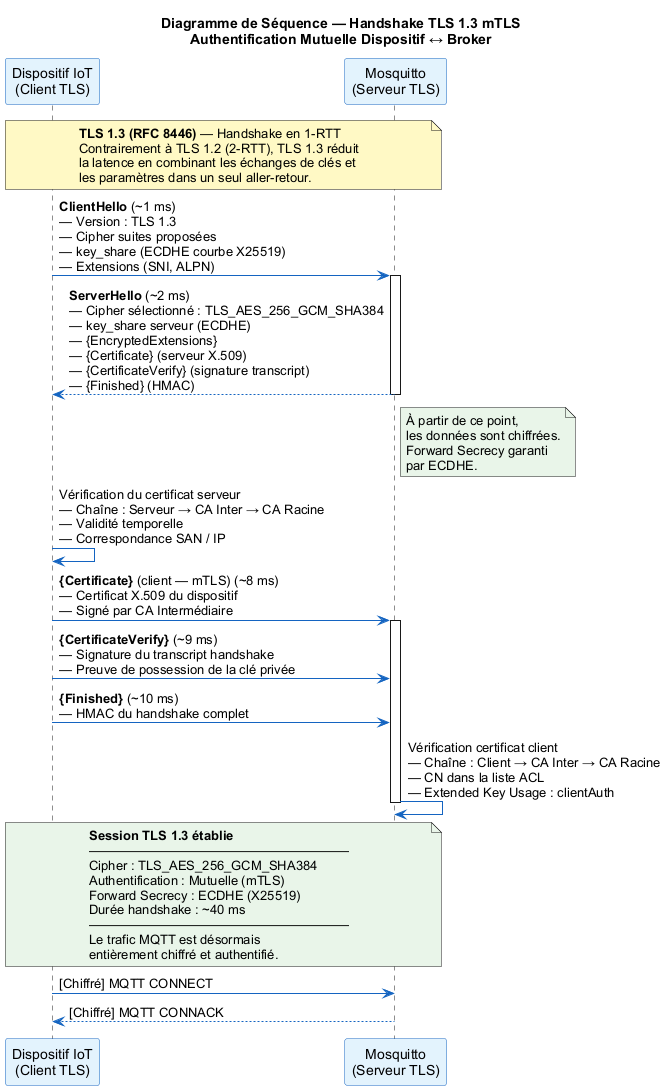
\includegraphics[width=0.7\textwidth]{diagrams/diag-tls-handshake.png}
  \caption{Handshake TLS~1.3 en mode mTLS (diagramme de séquence)}
  \label{fig:tls_handshake_etat_art}
\end{figure}

\section{Infrastructures à Clés Publiques pour l'IoT}

\subsection{Défis spécifiques à l'IoT}

La gestion des certificats dans un écosystème IoT présente des défis uniques~\cite{nist_sp800213} :
\begin{itemize}
  \item \textbf{Volume :} Des milliers à millions de dispositifs, chacun nécessitant un certificat unique.
  \item \textbf{Durée de vie courte :} Pour limiter l'exposition en cas de compromission.
  \item \textbf{Rotation automatisée :} Les dispositifs ne peuvent pas renouveler manuellement leurs certificats.
  \item \textbf{Révocation :} Les CRL ou OCSP doivent être accessibles même sur réseaux contraints.
\end{itemize}

\subsection{HashiCorp Vault comme PKI dynamique}

HashiCorp Vault est une solution open-source de gestion des secrets et de PKI dynamique~\cite{vault_pki}. Son moteur \texttt{pki} permet :
\begin{itemize}
  \item L'émission automatisée de certificats X.509 via API REST ou CLI.
  \item La définition de \textbf{rôles} avec des contraintes (TTL, CN autorisés, IP SAN).
  \item L'intégration avec des orchestrateurs (Kubernetes, Nomad) ou des scripts shell.
  \item La révocation immédiate et la génération automatique de CRL.
\end{itemize}

La figure~\ref{fig:pki_hierarchy_etat_art} présente le modèle de hiérarchie PKI à deux niveaux retenu dans notre architecture.

\begin{figure}[H]
  \centering
  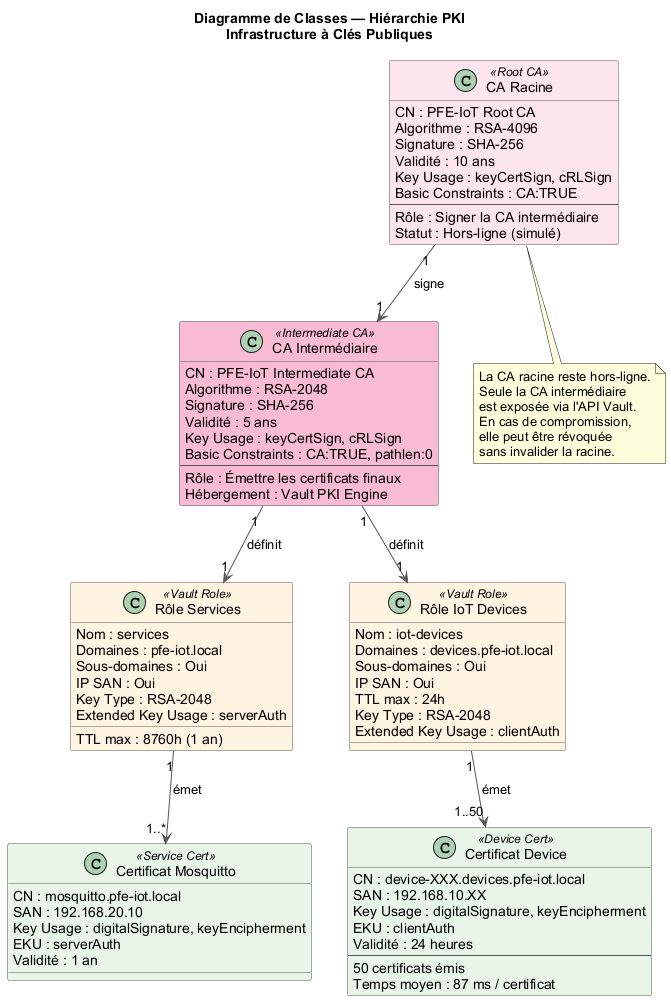
\includegraphics[width=0.75\textwidth]{diagrams/diag-pki-hierarchy.png}
  \caption{Hiérarchie PKI -- diagramme de classes (CA Racine, CA Intermédiaire, Rôles)}
  \label{fig:pki_hierarchy_etat_art}
\end{figure}

\section{Détection d'anomalies et SIEM}

\subsection{Suricata IDS}

Suricata est un moteur IDS/IPS open-source multi-thread supportant l'inspection en profondeur des paquets (DPI)~\cite{suricata_mqtt}. Il supporte nativement le protocole MQTT depuis sa version 6.0 (\texttt{app-layer-protocol: mqtt}), ce qui permet d'écrire des règles spécifiques aux topics et aux payloads MQTT.

\subsection{Wazuh SIEM}

Wazuh est une plateforme SIEM open-source issue du fork d'OSSEC~\cite{wazuh_docs}. Elle offre :
\begin{itemize}
  \item Un agent léger déployable sur Linux, Windows, macOS et conteneurs.
  \item Un moteur de règles configurable avec corrélation multi-sources.
  \item L'intégration native avec OpenSearch/Elasticsearch pour la visualisation.
  \item Des modules spécialisés pour Suricata, Docker, Kubernetes, AWS CloudTrail.
\end{itemize}

\subsection{Machine Learning pour la détection d'anomalies IoT}

Deux approches complémentaires ont été retenues :

\textbf{IsolationForest}~\cite{liu2008isolation} est un algorithme non supervisé basé sur la construction d'arbres d'isolation aléatoires. Les points anormaux, étant rares et distincts, sont isolés en un nombre minimal de partitions. Son avantage majeur est l'absence de nécessité d'étiquettes : il peut détecter des attaques inconnues.

\textbf{Random Forest}~\cite{breiman2001random} est un ensemble d'arbres de décision entraîné en mode supervisé. Il exploite les étiquettes disponibles pour apprendre les signatures spécifiques de chaque type d'attaque, atteignant des performances proches de la perfection sur des datasets équilibrés.

\section{Synthèse et positionnement}

\begin{table}[H]
\centering
\caption{Positionnement par rapport aux travaux existants}
\label{tab:positionnement}
\begin{tabular}{lcccc}
\toprule
\textbf{Solution} & \textbf{PKI complète} & \textbf{mTLS MQTT} & \textbf{IDS} & \textbf{ML détection} \\
\midrule
AWS IoT Core & \checkmark & \checkmark & $\sim$ & $\sim$ \\
Azure IoT Hub & \checkmark & \checkmark & $\sim$ & \checkmark \\
Eclipse Mosquitto (base) & $\times$ & Optionnel & $\times$ & $\times$ \\
Travaux académiques & Partiel & Partiel & Partiel & Isolé \\
\textbf{Cette architecture} & \checkmark & \checkmark & \checkmark & \checkmark \\
\bottomrule
\end{tabular}
\end{table}

Notre contribution se distingue par l'intégration verticale complète, du certificat dispositif jusqu'à la détection ML, dans un environnement simulé reproductible et entièrement open-source.
